\documentclass[conference]{IEEEtran}
%\documentclass[journal]{IEEEtran}
\usepackage{graphicx}
%\documentclass[]{article}

%\usepackage{draftwatermark}\SetWatermarkText{Not For Distribution}
%\SetWatermarkScale{2}\SetWatermarkLightness{0.85}

\newcommand{\ppv}{P_{pv}}
\newcommand{\pinv}{P_{inv}}

\title{Title}

\begin{document}

%\abstract{}

%\author{
%\IEEEauthorblockN{Daniel Soto}
%\IEEEauthorblockA{
%The Earth Institute\\
%Columbia University\\
%New York, NY 10027}
%\and
%\IEEEauthorblockN{Vijay Modi}
%\IEEEauthorblockA{
%Department of Mechanical Engineering\\
%Columbia, University\\
%New York, NY  10027}
%}

\maketitle

\begin{abstract}
Abstract.
\end{abstract}

\section{Introduction}

The cost of renewable and distributed energy systems must be
optimized to provide electricity to the customers beyond the
reach of the grid.

Communities in developing countries do not have easy access
to capital.
This constraint makes it necessary to optimize energy systems
for cost.
This work presents opportunities for efficiency and therefore
cost reduction in the areas of power conversion and storage.
These recommendations are based on data collected from customers
who have recently been provided with a near-grid-quality
electrical connection and are paying for that power on a
per kilowatt-hour basis.
There are many optimizations of system size in the literature
\cite{optimizations}.
This work adds to the literature by considering the effects
of the time of day of usage and the efficiencies of commonly
used inverters and batteries.

%We treat the hourly load profile and its effect on the
%generation and storage needed.
%We also observe for most of the systems that there is a wide variation
%in the system load with most power consumption in the evening.
%In a system that relies on an inverter, the inverter is run at a very
%inefficient operating point for much of the time.
%This lowers the overall efficiency of the system, increasing the
%necessary generation and storage costs.
%
%If the system is run inefficiently during the daytime, the inefficiency
%burden only impacts the amount of generation capacity needed.
%If the system is run inefficiently during the evening, both the
%generation and the storage costs are affected, multiplying the
%penalty.
%
%In this work we explore the interplay between consumption coincident
%with generation and consumption at different times from generation
%and quantify the impact on system costs.
%
%Two approaches to mitigation exist, the first is scheduling of loads
%to attempt to smooth consumption.
%Two of our sites have added refrigerators and we show the load duration
%curve with the addition of these devices and the effect on overall
%efficiency.
%
%The second approach is developing
%a power solution that is less sensitive to the variation in loads.
%We quantify the potential savings of each of these approaches.
%The approaches include parallel inverters, inverters with a
%standby mode, and DC distribution.
%
%When electricity is first delivered, use will likely be predominantly
%at nighttime.
%This means that there will be long periods of time where the power
%conversion electronics, usually inverters, are running at a low
%efficiency.
%This adds to the generation and storage burden of the system.
%
%We demonstrate this in a simple model where an assumed inverter curve
%is used and clear sky insolation is used for different daily
%loads.
%This is compared against a power conversion device with a flat
%efficiency curve.
%
%We argue for the development or adaptation of emerging technologies
%for the off-grid space.
%Some of these advanced technologies are cost competitive now.
%In this paper we describe some of the techno-economic
%details in the provision of standalone PV systems
%in rural areas.

\section{Microgrid and Data Description}
\subsection{Data collection}
We have installed 17 microgrid systems with remote connectivity
in Mali and Uganda \cite{ICTD}.
Each of these systems consists of a 1.4 kWp array of photovoltaic
panels with a 48 V, 360 Ah battery bank.
An MPPT charge controller handles battery charging and a
750 W inverter supplies the microgrid with 50 Hz, 220 V power.
Up to 20 customers are connected to these systems in a star
topology where each customer has a dedicated wire to the
central facility.
Each customer is metered by a commercially available device that
allows for energy measurement and reporting and a switch to
automatically connect or disconnect the consumer.
These systems send data on an hourly basis to a central server
using SMS messages.
Data is collected on the energy consumption of each household
as well as the AC energy consumption of the entire system.
From the solar controller, we measure and store hourly information
on the solar energy delivered to the system and the battery
voltage.

\subsection{Timeseries Description}
These messages allow us to create a database of timeseries
information from the customers.
For most customers, the peak power is consumed in the evening
as shown in Figure \ref{two-bulb-profile}.
Most of the customers have little or no usage during the day time.
The system however, uses about 50W to run the metering, computation,
and communication electronics giving a similar profile but with
a larger daytime use.

\begin{figure}[h]
\begin{center}
\includegraphics[trim = 0.0in 0.7in 0.0in 0.4in, clip, width=\columnwidth]
{figures/pchpp-ml03-217.pdf}
\end{center}
\caption{Customer exhibiting two bulb lighting load.
Each data point is the hourly load for a single day.
Multiple days are superimposed.
Points are transparent so that frequent measurements appear darker.
This customer displays two common evening power levels corresponding
to the use of one or two lightbulbs.
This not that this customer has very small power use during the day.}
\label{two-bulb-profile}
\end{figure}

We have provided two freezers that customers are using to
sell ice or frozen drinks.
The hourly profile for the household using this freezer
is shown in Figure \ref{freezer}.
These freezers draw a much larger amount of power than the
typical lighting load and have a lower variation when measured
on an hourly basis.

\begin{figure}[]
\begin{center}
\includegraphics[trim = 0.5in 0.8in 0.5in 0.9in, clip, width=\columnwidth]{figures/ml06-16.pdf}
\end{center}
\caption{Freezer load.}
\label{freezer}
\end{figure}

\subsection{Load Duration Curves}
If we sort the hourly power demand over a long time period, we
construct a curve called a load duration curve \cite{REEPS}.
A load-duration curve (Figure \ref{ldc}) shows this variation.
In the microgrid (ml07) that does not have a freezer, the most common
power level is less than 50W, which is well below the peak
efficiency of the inverter.
For the system that does have a freezer, the system spends the bulk
of its time consuming on the order of 200W, which is much closer
to the peak efficiency operating point of the inverter.
The inverter is sized so that the maximum customer load is safely
accommodated by the inverter.
However, there is a substantial efficiency penalty for operating the
inverter below the optimal point.

We can express these loads in terms of the capacity factor,
where the capacity factor is relative to the rated output
of the inverter.
Systems with high power variability will lose efficiency since
the system will often be operated outside of the range of
peak efficiency.

These systems have a 1.4 kWp solar array and an inverter rated
at 750W.

\begin{figure}[h]
\begin{center}
\includegraphics[trim = 0.0in 0.4in 0.0in 0.5in, clip, width=\columnwidth]{figures/two-ldc.pdf}
\end{center}
\caption{Load duration curve for two typical microgrid system,
including metering, computing, and computation.
Inverter and charge controller consumption is not included.
One system includes a significant daytime refrigeration load,
while the other does not.
}
\label{ldc}
\end{figure}

\subsection{Overall System Efficiency}

We can estimate an overall system efficiency from the
usage data and information from the solar controller
on photovoltaic energy generation.
This estimate of the overall efficiency of the system
is defined as power delivered by solar
power controller divided by the power delivered to the system.
We do not include the parasitic power consumed by the electronics.

Our data shows that as the capacity factor of the inverter
increases, the overall system efficiency improves.

The large variations in loads exhibited by these customers prompted
us to investigate the impact on system efficiency that these
loads are causing.
We pursued both a measurement of the systems and a simulation approach.

\begin{table}
\centering
\begin{tabular}{c c c}
Meter & System Utilization Factor & System Efficiency \\
\hline
ml03 & 0.38 & 0.62 \\
ml05 & 0.33 & 0.69 \\
ml06 (freezer) & 0.54 & 0.88 \\
ml08 (freezer) & 0.55 & 0.90 \\
\end{tabular}
\caption{System Utilization and system efficiency}
\label{efficiency}
\end{table}

In ML06, which has considerable daily load, we see an overall
efficiency of 0.89.
In ML05, with much less daily load, the overall efficiency
is 0.78.

\section{System and Simulation Description}

We examine the effect of load variation and alternate technologies
by creating a simulation of the system.
The model uses energy as the quanitity being modeled.
The simulation finds the minimum panel size and battery capacity
that will meet the demand assuming clear-sky radiation.
The model is intended to allow comparisons between systems and
load profiles rather than provide accurate guidance for system
sizes over a typical meteorological year.
The simulation takes as input the hourly load profile from a
set of customers.
In the following simulations we use both measured and simulated
loads.
Based on the hourly load profile, the energy in the battery
is simulated.
The battery is considered to be a simple energy storage device
with perfect efficiency during charging and an efficiency of
$\eta_B$ on discharge.
The panel size in the model is adjusted until the energy remaining
in the battery at the end of the simulation is equal to the
energy at the start of the simulation.
The minimum battery size is then the peak-to-peak variation
of the battery energy time series.
A time series trace is shown in Figure \ref{simulation}.

We can calculate the energy in the battery in discrete time
steps according to the following equation.
%
$$ E_B(t+\Delta t) = E_B(t)
                   + P_{charge} \cdot \Delta t
                   - \frac{P_{discharge} \cdot \Delta t}{\eta_B}
                   $$
%
Where $P_{charge}$ is the power flow when the photovoltaic
production is greater than the inverter demand and
$P_{discharge}$ is the power flow when the inverter demand
is greater than the photovoltaic power available.
They are given by the following equations.
%
$$ P_{charge} = \left\{
			  \begin{array}{rl}
			  0 & \pinv > \ppv \\
			  \ppv - \pinv & \pinv < \ppv
			  \end{array}
			  \right. $$
%
$$ P_{discharge} = \left\{
			  \begin{array}{rl}
			  \pinv - \ppv & \pinv > \ppv \\
			  0 & \pinv < \ppv
			  \end{array}
			  \right. $$
%
The power demanded by the inverter is calculated using the efficiency
of the inverter as a function of temperature according to
$$ \pinv = \frac{P_{AC}}{\eta_{inv}(P_{AC})} $$.

\begin{itemize}
\item $E_B(t)$ the battery energy available at time $t$
\item $\ppv$ Power produced by the PV panel
\item $\pinv$ Power demanded by the inverter
\end{itemize}

\begin{figure}[h]
\begin{center}
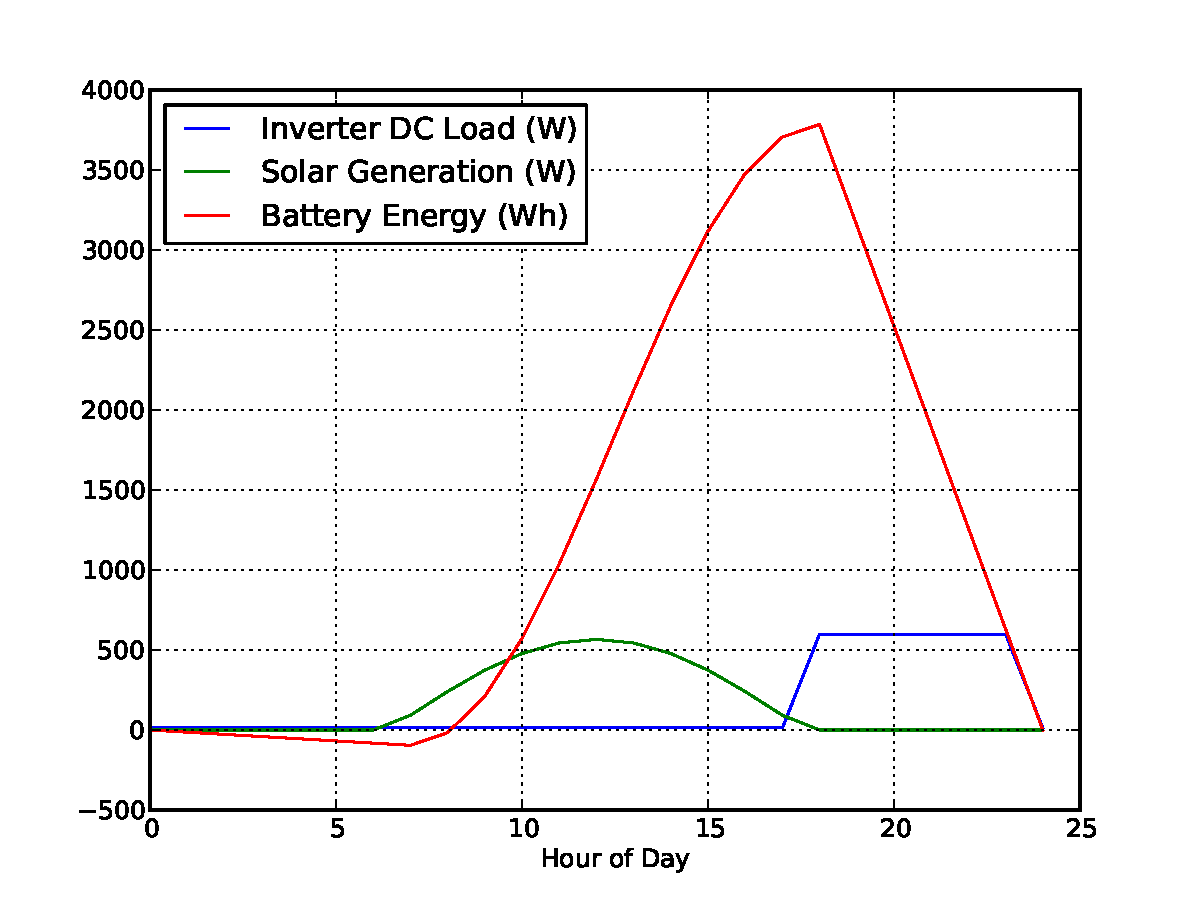
\includegraphics[trim = 0.0in 0.2in 0.0in 0.5in, clip, width=\columnwidth]{figures/simulation.pdf}
\end{center}
\caption{
Simulation.
}
\label{Graph of simulation output.}
\end{figure}

\begin{figure}[]
\begin{center}
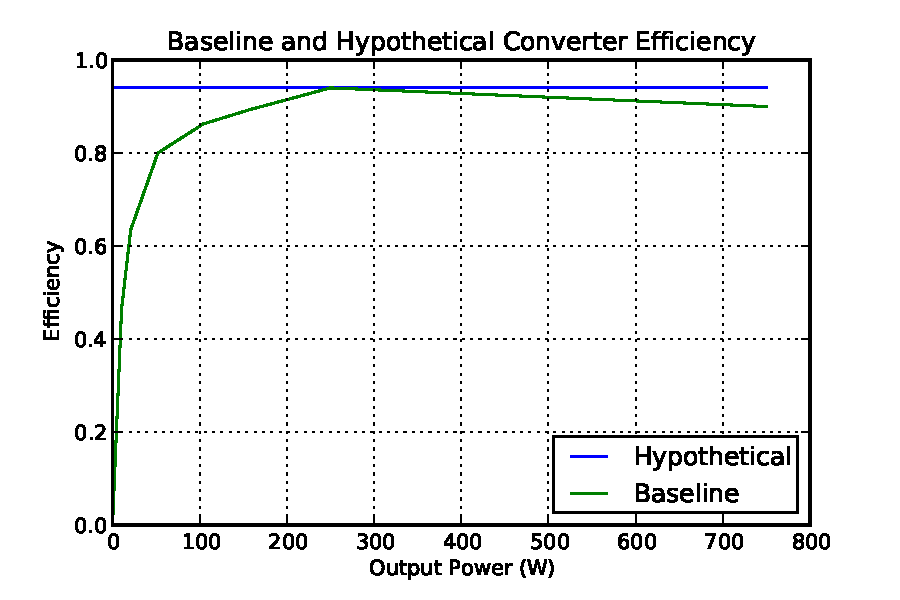
\includegraphics[width=\columnwidth]{figures/inverter_curves.pdf}
\end{center}
\caption{Efficiency curves for baseline and proposed system.}
\label{inverter_curves}
\end{figure}

\section{Simulation Results}

The simulation results compare the performance of hypothetical
systems to the baseline system and report potential improvements.

\subsection{Baseline System}
The simulated baseline system is based on the system we have
installed in the field.
The inverter efficiencies for this system are shown in Figure
\ref{inverter_curves}.
We assume a battery energy efficiency of 75\% round trip.

\subsection{Impact of time of load on system size}

To demonstrate the effect of the time of day that power
is consumed on the generation and storage capacity of the system.
We calculate the panel and battery size for four loads with
the same daily energy but occurring at different times of day.
The nighttime load has the entire day's load occurring between
6pm and midnight.
The daytime load occurs between 9am and 3pm and the constant
load is evenly spread across the entire day.
The village load uses a representative day from one of the
village microgrids and has a small constant load and a large
nighttime load.

Table \ref{load_type_impact}, shows the results of simulations
which demonstrate the variability of panel size and battery
size with the type of load.
During the day, current and power flows directly from the output of
the charge controller, through the inverter to the load.
This causes about a 10\% variation in panel area and a
nearly three-fold change in the minimum battery size needed.

\begin{table}
\centering
\begin{tabular}{c c c}
Configuration & Panel          & Minimum Battery \\
              & Area (m$^2$)   & Size (kWh)      \\
\hline
Baseline System, Daytime Load   & 2.83 & 0.76 \\
Baseline System, Nighttime Load & 2.94 & 3.88 \\
Baseline System, Constant Load  & 3.05 & 2.46 \\
Baseline System, Village Load   & 3.08 & 2.93 \\
\end{tabular}
\caption{Impact of load time-of-day on system size.
Loads are normalized to 3.0 kWh per day.}
\label{load_type_impact}
\end{table}

\subsection{Inverter Efficiency}

A typical inverter is inefficient at loads below its
preferred operating point.
If the load is usually close to this high efficiency
point, the lower efficiencies at low power are not important.
If however, as we observe, there is a high variability
in the power output where daytime loads are very small
but evening loads are greater, this inefficiency can have
a significant impact.

To demonstrate this effect, we run our simulation with
a hypothetical power conversion device that has an
efficiency equal to the peak efficiency of the baseline
inverter at any power level.

Table \ref{table_inverter} shows greater reductions
in the generation and storage needed for loads that
are often below peak, such as the measure village load
and the continuous load.

\begin{table}
\centering
\begin{tabular}{c c c}
Configuration & Panel          & Minimum Battery \\
              & Area (m$^2$)   & Size (kWh)      \\
\hline
flat day        & 2.36 & 0.83 \\
flat night      & 2.45 & 3.36 \\
flat continuous & 2.30 & 1.86 \\
flat village    & 2.33 & 2.25 \\
\end{tabular}
\caption{Impact of inverter non-ideality on system size}
\label{table_inverter}
\end{table}

\subsection{Battery Chemistry}

The initial battery cost is given by

$$ C_B = E_{storage} \frac{1}{\eta_B} \frac{1}{DOD_{optimal}} c_B $$

Where $E_{storage}$ is the storage necessary, $\eta_B$ is the
round trip energy efficiency, $DOD_{optimal}$ is the desired
operating point of the battery for long life, and $c_B$ is the
initial cost of the battery per kWh.
A very important metric however is the life cycle cost of the 
battery replacement which depends on the cycle life of the battery.

New battery chemistries could reduce the fraction of investment
that goes toward storage of electricity.
The incumbent battery technology is sealed lead acid.
Emerging technologies of interest are Lithium Iron Phosphate
and Lead Carbon.

Relative to sealed lead acid batteries, LiFePO batteries 
have better cycle life, higher specific cost, and better
turnaround efficiency.
PbC batteries are not yet mature but have improved cycle
life and likely similar specific cost and turnaround
efficiency.
We simulate the impact of these on system size and total cost
in Table \ref{table_battery}.
For the case of typical village data, the lifetime cost of 
lead acid and LFP are similar.
If PbC batteries are able to maintain their cost while
improving cycle life, they will provide a clear improvement
in the life-cycle cost.

\begin{table}
\centering
\begin{tabular}{@{} l %{0.3\columnwidth}
                c %p{0.3\columnwidth}
                c %p{0.3\columnwidth} 
                c @{}}

Battery Chemistry & Initial Cost & Lifetime & Optimal \\ 
                  & (USD/kWh)    & (yr)      & DOD\\
Lead Acid (LA)               & \$140  & 2  &  50\%  \\
Lithium Iron Phosphate (LFP) & \$1000 & 6  & 100\%   \\ 
Lead Carbon (PbC)            & \$140  & 6  &  50\%   \\
\end{tabular}
\caption{Battery Assumptions.}
\label{table_battery_assumptions}
\end{table}

\begin{table*}[!t]
\centering
\begin{tabular}{ c  c
                 c 
                 c c}
Load Type & Battery & Panel          & Minimum Battery & Battery NPV\\
                    & Area (m$^2$)   & Size (kWh)      \\
\hline
typical day & lead acid          & 2.97 & 0.76 & 1305 \\
typical day & LFP                & 2.83 & 0.76 & 1824 \\
typical day & lead carbon        & 2.97 & 0.76 & 514 \\

typical night & lead acid        & 3.69 & 4.92 & 8421 \\
typical night & LFP              & 2.94 & 3.88 & 9338 \\
typical night & lead carbon      & 3.69 & 4.92 & 3312 \\

typical continuous & lead acid   & 3.52 & 3.08 & 5281 \\
typical continuous & LFP         & 3.05 & 2.46 & 5931 \\
typical continuous & lead carbon & 3.52 & 3.08 & 2077 \\

typical village & lead acid      & 3.64 & 3.66 & 6270 \\
typical village & LFP            & 3.08 & 2.93 & 7043 \\
typical village & lead carbon    & 3.64 & 3.66 & 2466 \\
\end{tabular}
\caption{Simulation results for battery chemistries.
Net present value is calculated at 7\% over 20 year 
time horizon.}
\label{table_battery}
\end{table*}


\section{Discussion}
Here we discuss what methods are available to mitigate the
load variations and increase efficiencies.

\subsection{Mitigating Load Variation}
Systems with better no-load performance should be used to counteract
the problem of efficiency at the lower end.

Two solutions exist for this problem, the first is to remove
the constant loads (meter electronics, communication, and
computing) from the inverter.
This could allow an inverter to operate in a power-down or
search mode for most of the time and then switch on only
to service loads.

\subsubsection{Slaved inverters}
A chain of inverters that turn on in a cascaded fashion could
be more efficient.

\subsubsection{Inverters with Standby Mode}
The standby loss could be low but an small use will energize the
entire system.

\subsubsection{DC Distribution}

Since both the generation and consumption of electricity in our
sites is in the form of DC electricity, it is natural to
question the necessity of the inverter.
In addition to inefficiency of conversion from DC to AC at the
generation side and from AC to DC at the consumption side,
these DC loads have less than unity power factor which further
lowers the efficiency of the inverter.
In areas where connection to the grid is extremely unlikely
in the future, an all DC distribution system is worthy of
serious consideration.

If the efficiency curve of a DC/DC converter were favorable,
a high-voltage direct current (HVDC) distribution scheme could
be used.
Our testing of a 48 VDC to 12 VDC converter is over 80\% for
the range of power of interest.
The no-load dissipation for this device was below our measurement
capacity of 0.5W.


\subsection{Battery Chemistry}

% lithium iron phosphate
% 0.40-2 USD/Wh
% 2000 cycles
% optimal DOD 100%

% lead acid
% 0.14 USD/Wh
% 500-800 cycles
% optimal DOD 50%

% lead carbon
% 
% 2000 cycles @ 100% DOD

\subsection{Distributed Storage}
Another possibility is local storage at the home with a small inverter
that the customer only switches on during times when power
is needed.
This reduces the standby load to zero but likely adds to the
fixed cost of the system.

\subsection{Load Shaping}

A strategy for improving the overall efficiency of the system
is to schedule consumer loads such that the load profile is
more constant.
In the context of remote villages, the initial loads are mostly
lighting and entertainment in the evening and have very limited
capacity for rescheduling.
Another strategy is to create daytime loads.


\subsection{Using Real vs Apparent Power}
Almost all loads used by customers in our microgrids have power
factors below one.
These switching power supplies negatively affect inverter efficiency
and thus the battery supply.
To properly account for the customer wear and tear on the battery
it likely makes more sense to charge for apparent power or for
real power adjusted by power factor.

\section{Summary}
Hourly demand data for newly electificed communities has been gathered.
We find that improving no-load and low load power consumption of the
inverter can reduce storage and generation needs.

technology \& cost improvement from baseline \\
slaved inverters \& xx\% \\


\begin{thebibliography}{1}
\bibitem{optimizations}
Z Wissem, K Gueorgui, K H\'edi,
Modeling and techinical--economic optimization of an autonomous
photovoltaic system,
Energy, Vol. 37, 2012 pp. 263-272
(doi:10.1016/j.energy.2011.11.036)
\bibitem{ICTD}
D.~Soto, SharedSolar. ICTD 2012.
\bibitem{REEPS}
G.~Masters,
"Renewable and Efficient Electric Power Systems",
Wiley Interscience,
2004
\end{thebibliography}


\end{document}

%---------------------------------------------------------------------------%
%---------------------------------------------------------------------------%
%---------------------------------------------------------------------------%
%---------------------------------------------------------------------------%
%---------------------------------------------------------------------------%
%---------------------------------------------------------------------------%
%---------------------------------------------------------------------------%
%---------------------------------------------------------------------------%
%---------------------------------------------------------------------------%
%---------------------------------------------------------------------------%
%---------------------------------------------------------------------------%
%---------------------------------------------------------------------------%



We have measured the load patterns of users and have generated
load-duration curves over a N-day period.
From this curve, (Figure \ref{ldc}) we estimate the overall
efficiency of the inverter.
$$ \sum p_i / \eta_i $$
The overall inverter efficiency is much lower than its rated
efficiency because the inverter is operated for so much time
at a low fraction of its capacity.


%$$ \ppv = insolation \cdot array size \cdot array efficiency
%         \cdot controller efficiency $$


We can simulate the effective inverter efficiency for a given
load profile and inverter curve.

$$ \eta_{effective} = \frac{\sum P_{AC} \cdot \Delta t}
                          {\sum P_{AC} /\eta_{inv} \cdot \Delta t} $$

While lithium batteries are a factor of XX more expensive
than lead-acid batteries based on the capacity of the battery
(USD/kWh), the cost per delivered watt-hour of electricity
over the lifetime of the battery is comparable.
Additional economic improvement is gained by lower weight
for shipping and improved round trip efficiency which lowers
both the battery capacity and the generation capacity when nighttime
loads are needed.
